\section{Metodología}
\subsection{Análisis de datos}
Para poder entrenar un algoritmo de aprendizaje profundo se requiere un conjunto de datos extensos. Este conjunto debe poder representar de la mejor manera posible el fenómeno que se quiere procesar. Además, se debe poder asegurar que todas las instancias que componen la base de datos tengan características homogéneas que se adecuen a los procesos subsiguientes. 

Para este trabajo, es necesario partir de un conjunto de datos conformados por dos tipos de elementos principales: Respuestas al impulso, y grabaciones de voz. Con estos elementos, es posible generar instancias que comprendan información de audio con reverberación y su correspondiente versión anecoica, siendo esta última la que un sistema de dereverberación tiene como objetivo.

Además, se debe tener en cuenta que se busca formar tres grandes conjuntos de datos: conjunto de entrenamiento, conjunto de validación y conjunto de prueba. Las características de estos conjuntos deberán variar de acuerdo al propósito de cada uno para lograr optimizar cada etapa, o bien, para evaluar ciertos aspectos de estos procesos.    


\subsubsection{Base de datos de respuestas al impulso}

Para este trabajo se utilizan respuestas al impulso reales y simuladas. 

Las respuestas al impulso reales se obtienen del conjunto de datos C4DM \cite{rir_reales}. Este conjunto consiste en una colección de respuestas al impulso que fueron medidas en tres recintos: una sala multipropósito con aproximadamente 800 asientos, un edificio victoriano construido en 1988 originalmente diseñado para ser una biblioteca, y una sala de clases de una universidad. Las mediciones fueron realizadas utilizando la técnica del barrido frecuencial \cite{sinesweep}. Para todas estas respuestas al impulso, el tiempo de reverberación es de aproximadamente 2 segundos. 

En cuanto a las respuestas al impulso simuladas, se utiliza la librería de Python 'PyRoomAcoustics' \cite{pyroom} para generarlas. Esta librería brinda un software de generación de respuestas al impulso basado en el método de fuente imagen  \cite{ISM}. El algoritmo está implementado en el lenguaje de programación C, permitiendo una rápida simulación de la propagación del sonido en recintos poliédricos. Los parámetros que se deben indicar a la hora de generar una respuesta al impulso son: 

\begin{itemize}
\item Dimensiones del recinto (largo, ancho y alto).
\item Posiciones de fuente y receptor, en coordenadas tridimensionales.
\item Coeficientes de absorción de las superficies.
\item Orden máximo de reflexiones a computar.
\end{itemize} 

Para generar los datos se proponen dos recintos, el primero de dimensiones $8m\: x\: 6m\: x\: 4m$ que se denominará 'Recinto 1' , el segundo de dimensiones $6m\: x\: 4m\: x\: 3.5m$ que se denominará 'Recinto 2'. En la figura \ref{fig:recintos} se pueden visualizar ambos recintos generados. 

\begin{figure}[H]
	\centering{}
	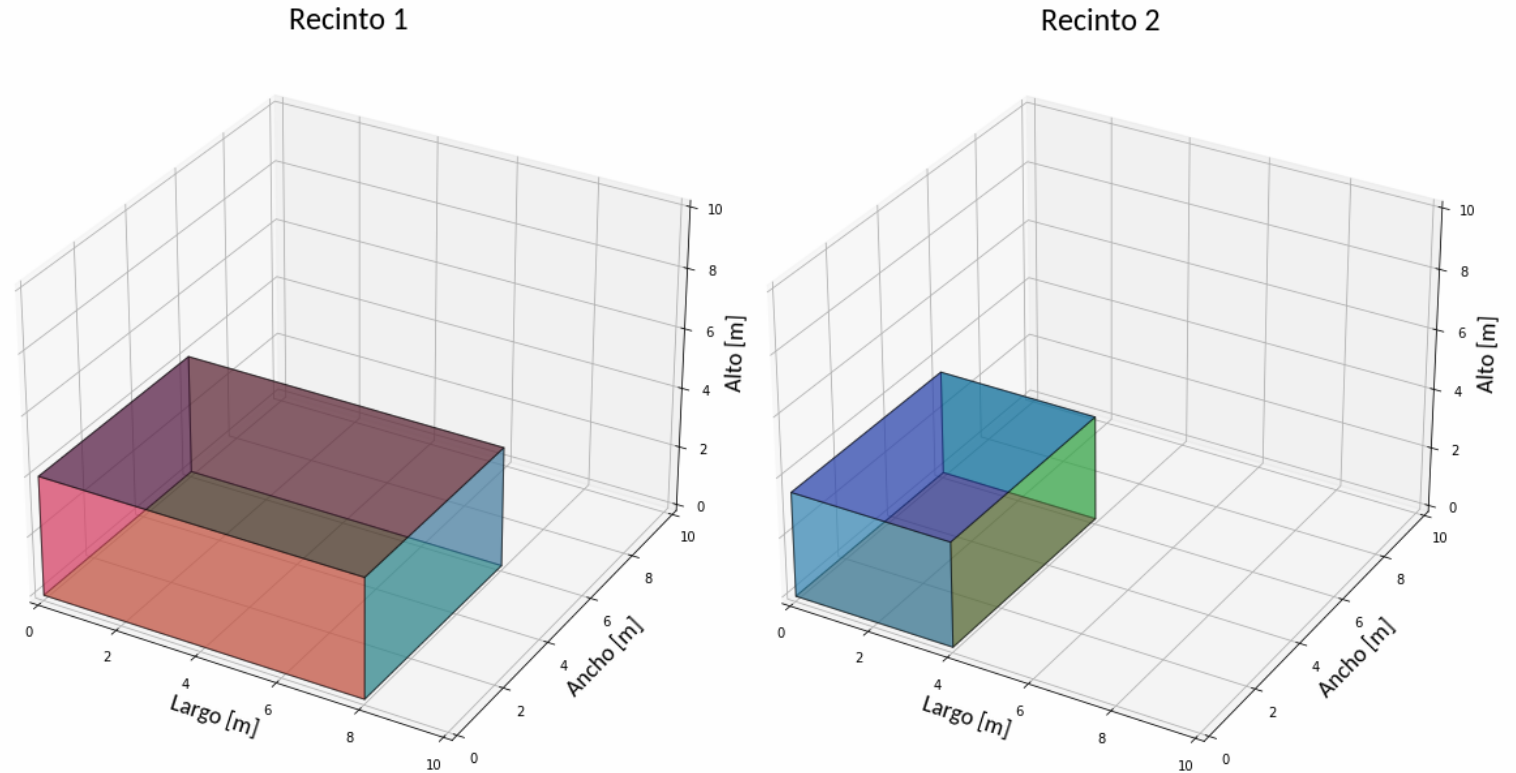
\includegraphics[scale=0.3]{recintos.png}
	\caption{Recintos generados para la simulacion de respuestas al impulso}
	\label{fig:recintos}
\end{figure}

Para controlar los demás parámetros que refieren a las condiciones del recinto, se subordina el orden máximo de reflexiones y los coeficientes de absorción a un tiempo de reverberación esperado. Esto es, teniendo un cierto recinto se determina un valor de tiempo de reverberación T60 inicial. Este se utiliza para estimar un valor de un coeficiente de absorción promedio mediante la ecuación de Sabine y también en base a este tiempo se determina el orden de reflexiones necesario para poder representar la reverberación. 
Por último, las posiciones de fuente y receptor se generan aleatoriamente para poder generar diferentes respuestas al impulso a partir de un mismo recinto. De esta manera, los datos que se deben determinar son las dimensiones del recinto, un tiempo de reverberación inicial y la cantidad de respuestas al impulso que se quiere generar. 


\subsubsection{Bases de datos de señales del habla}

Las señales del habla necesarias para formar los pares anecoico-reverberados se obtienen de la librería LibriSpeech \cite{librispeech} la cual consiste en un conjunto de datos que reúne 100 horas de audio correspondientes a lecturas en idioma inglés. Los datos corresponden a programas tipo audiolibros. Las señales poseen bajo nivel de reverberación, y provienen de una aplicación en la cual la inteligibilidad es primordial, lo cual hace que esta base de datos sea adecuada para utilizarse en este trabajo.

\subsubsection{Pre-procesamiento de datos}

Partiendo de audios de voz y respuestas al impulso, el modelo de red neuronal propuesto requiere generar instancias de espectrogramas de magnitud y máscaras ideales para poder entrenarse. Para conseguir esto, se programa una cadena de procesamiento automatizada que realice esta transformación de los datos de entrada. 
En primer lugar se controla la uniformidad de frecuencias de muestreo aplicando las transformaciones de aumentación o decimado cuando sean requeridas. Se decide trabajar con una frecuencia de muestreo de $16000$ muestras por segundo, considerando que se tratan con señales de voz que concentran su información por debajo del límite de representación frecuencial de $8000 Hz$ impuesto por esta decisión. 
Luego, los audios de voz se convolucionan con las respuestas al impulso para formar pares de señales con y sin reverberación. El resultado de la convolución se recorta para descartar el retardo generado por la convolución, haciendo que los pares de señales sean sincrónicas. Luego, se toman ventanas rectangulares de $32640$ muestras, lo que equivale a segmentos de audio de $2,04$ segundos para la frecuencia de muestreo utilizada. Lo siguiente es aplicar la transformada de corto término de Fourier tanto a la señal limpia como a la señal convolucionada. La transformada se aplica con una ventana de $512$ muestras y un salto de $128$ muestras lo cual equivale a un solapamiento del $75\%$. Esto permite la correcta reconstrucción de la señal al antitrasformar. Se obtienen espectrogramas complejos, a los cuales se les calcula la magnitud, descartando la información de fase. Además, se aplica una normalización para acotar el dominio en valores que sean convenientes para el algoritmo de  aprendizaje posterior. Con las magnitudes de los espectros anecoicos y reverberados, se calculan máscaras de amplitud ideales y luego se comprimen aplicando una función tangencial hiperbólica para la cual se definen los parámetros $Q=1$ y $C=0,5$. Finalmente, las instancias finales de este proceso son en el espectro de magnitud de la señal con reverberación (que corresponde a la variable de entrada de la red neuronal) y la máscara de magnitud ideal comprimida (que corresponde a la salida de la red, es decir, el objetivo que el modelo busca estimar). Ambas instancias tienen las mismas dimensiones, que corresponden a $256$ cuadros temporales y $257$ valores posibles de frecuencia (se conserva solo la parte positiva del espectro frecuencial simétrico). Por último, se descartan los puntos correspondientes al valor máximo de frecuencia. Esto se realiza para obtener dimensiones finales de $256x256$ lo cual facilita el proceso de compresión y expansión de los espectros al ser dimensiones múltiplos de $2$. Se descarta la frecuencia más alta ya que por la característica de la fuente  no contendrá información crucial para la representación.  

Cabe destacar que debido a este preprocesamiento aplicado, a la hora de evaluar el modelo se deberán aplicar una serie de procesos previos sobre el audio a procesar. Mas precisamente, se deberá segmentar el audio y obtener espectros de magnitud de la STFT respetando los mismos parámetros que en el preprocesamiento. Luego, como la salida de la red es una máscara de amplitud comprimida, se debe descomprimir esta máscara, aplicarla sobre el espectro reverberado y luego combinar el espectro de amplitud modificado resultante con la fase original de la señal para poder finalmente obtener la información de audio de salida a través de la aplicación del algoritmo de Griffin-Lim.  


\subsection{Modelo propuesto}

El modelo propuesto se basa en una arquitectura de red neuronal completamente convolucional tipo 'autoencoder' inspirada en el trabajo de Ernst et. al.\cite{FCN}. Más precisamente, un autoencoder es una estructura que tiene como objetivo aprender niveles de representación de la información de entrada, para luego poder reconstruir una instancia similar descartando la información no deseada o considerada "ruido". En este caso, la señal no deseada corresponde a la reverberación. El esquema básico del algoritmo se puede observar en la figura \ref{fig:autoencoder}, donde la variable $x$ representa a las variables de entrada, e $y$ representa la variable de salida. 

\begin{figure}[H]
	\centering{}
	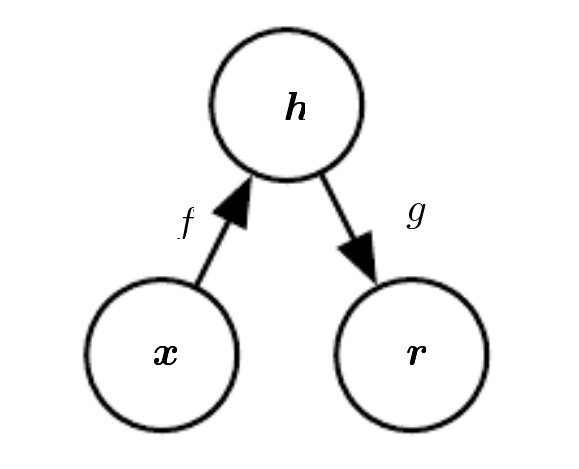
\includegraphics[scale=0.3]{autoencoder.png}
	\caption{Estructura general de un autoencoder.}
	\label{fig:autoencoder}
\end{figure}

El esquema se compone de tres partes fundamentales: 
\begin{itemize}
\item Una función de codificación $f$ en donde las dimensiones de la variable de entrada se comprimen y las características más relevantes son aprendidas. Esta función realiza el mapeo de la variable de entrada al espacio latente. 
\item Un espacio latente $h$ (o espacio de representación), en donde se concentran las representaciones internas aprendidas a partir de la compresión de la variable de entrada. 
\item Una función de decodificación en donde se aplica el proceso inverso que en la codificación, expandiendo las dimensiones tomadas del espacio latente para formar una representación que minimice el error de reconstrucción. 

\end{itemize}

El sistema propuesto consiste en la estimación del espectro de la señal anecoica a partir del espectro de la señal reverberada. Para conseguirlo, en lugar de hacer un mapeo directo entre ambos espectros, se opta por estimar una máscara de amplitud. Se decidió trabajar con máscaras ya que estudios previos demostraron que con este método se obtienen mejores resultados que realizando estimaciones de mapeos directos entre dos espectros. Para trabajar con espectros, las señales de entradas se transforman al dominio temporal-frecuencial a partir de la transformada de Fourier de corto término. Se utiliza una ventana temporal de 512 muestras, con un solapamiento del 75\%. 
La estructura de red neuronal utilizada consiste en una U-NET con conexiones de saltos, inspirada inicialmente en \cite{FCN}. Este tipo de estructuras consiste en tomar mapas bidimensionales de entrada y a partir de la aplicación sucesiva de capas convolucionales con valores de salto mayor a 1, reducir la dimensionalidad del mismo e ir aumentando el número de filtros utilizados por la capa convolutiva. Un esquema básico de está estructura se puede ver en la figura \ref{fig:unet}, en donde se puede ver que las dimensiones de las capas siguen una forma de 'U', lo cual le da el nombre a estas estructuras.

\begin{figure}[H]
	\centering{}
	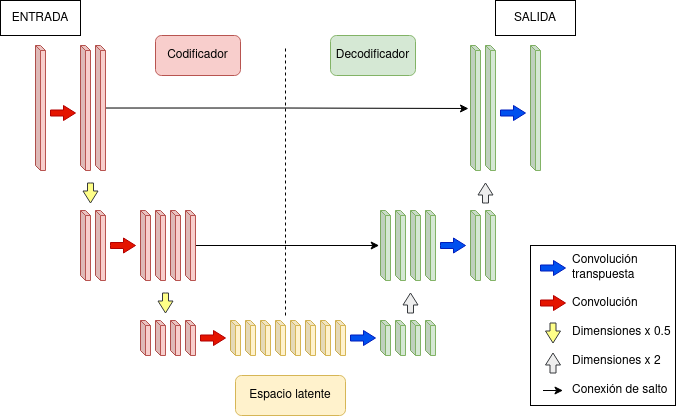
\includegraphics[scale=0.3]{unet.png}
	\caption{Esquema básico de una red tipo 'U-NET'.}
	\label{fig:unet}
\end{figure}

A medida que se avanza en el modelo, el tamaño del espectro de entrada va disminuyendo y la cantidad de filtros utilizados va aumentando. Esta primera parte se puede pensar como un codificador, ya que el sistema esta tomando información del espectro de manera jerárquica.  Este proceso se realiza sucesivamente hasta que la imagen de entrada alcanza una dimensión de 1x1. Luego, prosigue una etapa de decodificación en la cual se aplica el proceso inverso. Esto es, la dimensión del espectro se va aumentando con capas convolutivas transpuestas de saltos mayores a 1, y la cantidad de filtros utilizados va disminuyendo. Esto se repite hasta que las dimensiones del espectro sean las mismas que tenía a la entrada del codificador. Mediante este esquema de U-NET y el efecto del cuello de botella de las dimensiones, se consigue que la estimación de cada pixel de la imagen resultante esté condicionado por todos los pixeles que componen la imagen de entrada. Se puede decir entonces que la estimación de cada punto del espectro final depende de todo el espectro de entrada, y no solo de una región determinada. 

Para poder pasar información de manera más directa desde el decodificador hacia el codificador, se implementan conexiones de salto. La conexión de salto consiste en concatenar la salida de una capa del codificador con una capa del decodificador. Para poder hacerlo, la dimensión de concatenación (en este caso, las dimensiones del espectrograma) deben ser las mismas. De esta manera se logran decodificaciones más precisas. 




Una representación gráfica del modelo final implementado se puede apreciar en la figura \ref{fig:modelo}. En cada capa se indican tres valores, donde el primero representa la dimension temporal, el segundo la dimension frecuencial y el tercero el numero de canales. En las primeras capas, las dimensiones se reducen a la mitad en cada instancia debido al uso de un desplazamiento de paso 2 en los filtros convolucionales, lo que realiza la compresión de la información. En las capas subsiguientes, las dimensiones sufren el efecto contrario hasta volver a obtener las dimensiones originales. Este tipo de estructura tiende a perder información importante de bajo nivel durante el proceso de compresión. Como por lo general las variables de entrada y de salida comparten información estructural, se puede mejorar el funcionamiento de estas estructuras implementando conexiones entre las capas del codificador y el decodificador. Esto quiere decir que los mapas de características de las capas que conforman el codificador se van a concatenar directamente con los mapas de características en el decodificador, es decir, la salida de la capa $i$ se concatena con la salida de la capa $N-i$ donde $N$ es el número de capas. Estos saltos evitan que las activaciones pasen por el cuello de botella permitiendo la propagación de esta información estructural que estas estructuras tienden a perder. 

\begin{figure}[H]
	\centering{}
	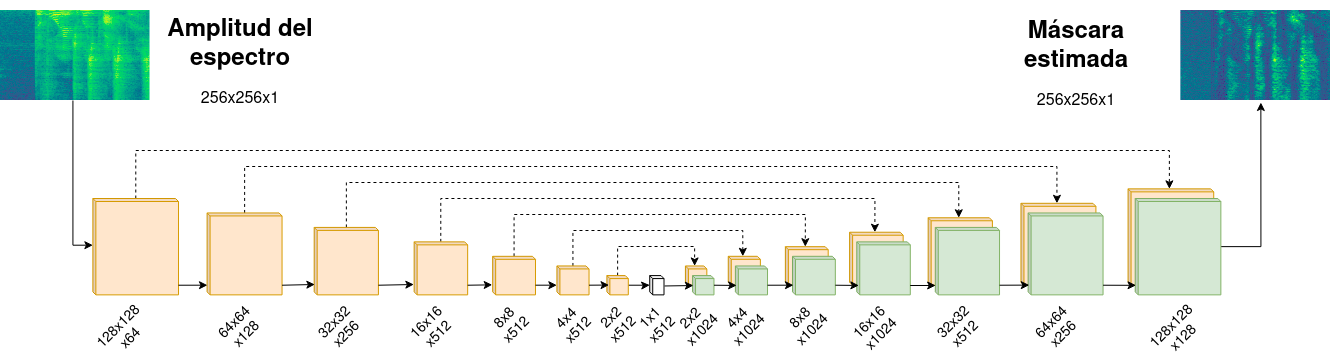
\includegraphics[scale=0.35]{modelo_red.png}
	\caption{Modelo de red neuronal convolucional implementado}
	\label{fig:modelo}
\end{figure}

De esta forma, el modelo realiza una compresión de los datos de entrada, buscando minimizar el error en la reconstrucción al comparar con las instancias que se le presentan como objetivo. 
Para este caso particular, las entradas del modelo son espectrogramas, es decir, valores en el dominio tiempo-frecuencia. Las dimensiones del espectrograma de entrada son comprimidas hasta llegar a dimensiones de $1x1$ y luego son expandidas nuevamente, lo que produce un aumento de los campos perceptivos que permite propagar información global tanto en tiempo como en frecuencia. Esto significa que el cómputo de cada pixel de salida se verá influenciado por la totalidad del espectrograma de entrada. Estudios previos demostraron que la estimación directa de espectros, o lo que es equivalente, el mapeo frecuencial-temporal genera resultados menos precisos comparado con aquellos modelos que en lugar de estimar espectros estiman máscaras espectrales\cite{mask_vs_map}. Por esto, las entradas del modelo son espectrogramas correspondientes a señales con reverberación, y las salidas u objetivos son máscaras de amplitud previamente calculadas en una etapa de preprocesamiento. 

\subsection{Especificaciones de la arquitectura implementada}

Como se indicó anteriormente, esta arquitectura se basa en el entrenamiento de un modelo completamente convolucional. Sin embargo, la etapa de codificación y decodificación requieren evaluar ciertos detalles a la hora de su implementación. 

En la etapa de codificación, la primera capa consiste en una capa convolucional utilizando una activación del tipo Leaky-Relu con una pendiente de $0,2$. Se escoge esta activación por sobre la rectificación lineal debido a que es favorable frente al problema de desvanecimiento de gradiente, lo cual puede ser un problema al trabajar con una arquitectura de red tan profunda. Luego, las seis capas subsiguientes son también capas convolucionales con la misma función de activación pero con el agregado de que implementan normalización por lotes. Finalmente, la última capa de esta etapa es convolucional con normalización por lotes y función de activación ReLU. 

En la etapa de decodificación es importante tener en cuenta que el tamaño de los campos perceptivos de las capas deben ser un múltiplos enteros del tamaño de salto para que no se produzcan artefactos indeseados durante el proceso inverso al cuello de botella que ocurre al utilizar capas deconvolutivas con tamaño de salto mayor a $1$. Sin embargo, aun teniendo esto en consideración, las capas de deconvolución pueden generar artefactos indeseados. En lugar de utilizar capas convolutivas se opta por implementar una combinación de dos capas consecutivas: en primer lugar una capa que aumente las dimensiones del espectrograma generando nuevos puntos a partir de una interpolación entre los valores mas cercanos, y luego una capa convolutiva. De esta manera se obtiene el efecto del aumento de dimensiones junto con el análisis convolutivo. Esta deconvolución se combina con un drop-out del 50\% y una función de activación ReLU en las primeras tres capas del decodificador. Luego, continuan 4 capas idénticas pero omitiendo el drop-out. Finalmente, la última capa del decodificador que a la vez es la capa de salida de la red consiste también en una deconvolución sin drop-out pero utilizando una función de activación tangencial, lo que significa que los valores de salida estarán acotados en el intervalo $[-1, 1]$.
En todas las capas convolucionales y deconvolucionales se utiliza un tamaño de filtro de $6x6$ y un tamaño de salto igual a $2$. 
Finalmente, la función de costo utilizada para evaluar las predicciones realizadas por el modelo frente a las máscaras ideales en la salida es el error cuadrático medio (MSE) el cual se expresa en la ecuación \ref{eqn:mse} y para la optimización se utilizó el algoritmo de estimación adaptativa de momento (ADAM) \cite{adam} con un valor de tasa de aprendizaje de $0,001$. 

\begin{equation}
\label{eqn:mse}
	L_{MSE} = \sum_{i=1}^{N-1}\overline{(M_{i}(t,f) - \hat{M}_{i}(t,f))^{2}} 
\end{equation}

\subsection{Manejo de datos a evaluar}
En este trabajo se ponen a prueba cuestiones relativas al manejo de datos utilizados para entrenar el algoritmo de aprendizaje profundo. Las pruebas se diferencian entre combinaciones entre datos simulados o reales, y en el ordenamiento de la complejidad de los datos durante el entrenamiento. 

En primer lugar, como se cuenta con respuestas al impulso reales y simuladas, se prueban combinaciones de estos datos a la hora de formar los diferentes conjuntos requeridos para el entrenamiento (conjunto de entrenamiento y conjunto de prueba). A la hora de formar los conjuntos, se debe poder conseguir una determinada dispersión de ciertos descriptores acústicos para poder asegurar que el conjunto es representativo de las distintas variantes posibles en el efecto de la reverberación. Para analizar esta cuestión se decide trabajar con los parámetros tiempo de reververación medio $TR_{mid}$ y relación directo-reverberado $DRR$. Estos descriptores son fácilmente controlables en las respuestas al impulso simuladas, debido a que se pueden controlar los parámetros en el algoritmo que las genera. Sin embargo, obtener esta heterogeneidad puede ser un problema al tratarse de respuestas al impulso reales debido a la escasez de bases de datos extensas. Para resolver esta cuestión se aplican procesamientos propuestos en \cite{aumentacion} para lograr una aumentación de datos y poder formar un conjunto representativo de respuestas al impulso reales. 
Teniendo en cuenta esto, se definen como se va a conformar los conjuntos de datos de entrenamiento y de prueba para cada evaluación. Cabe aclarar que el conjunto de validación se conforma tomando una porción del conjunto de entrenamiento. Entonces, las pruebas a realizar quedan definidas por las distintas combinaciones entre datos simulados y reales y los diferentes conjuntos de datos como se muestra en la tabla \ref{Tab:pruebas}. 

\begin{table}[]
\caption{Conformación de los distintos conjuntos de datos utilizados.}
\centering
\label{tab:pruebas}
\begin{tabular}{c|c|c|c|c}
                       & Prueba 1     & Prueba 2  & Prueba 3     & Prueba 4     \\ \hline
Conjunto de validación & RI simuladas & RI reales & RI simuladas & RI reales    \\
Conjunto de prueba     & RI simuladas & RI reales & RI reales    & RI simuladas
\end{tabular}
\end{table}

Para formar el conjunto de respuestas al impulso simuladas se utilizan 3 tiempos de reverberación principales: $0,5 s$ como reverberación baja, $0,75 s$ como reverberación media y $1,0 s$ como reverberación alta. Partiendo de estos tiempos, se generan 30 respuestas al impulso para cada uno, resultando en un total de 90 respuestas al impulso con tiempos de reverberación de entre aproximadamente $0.5$ segundos a $1$ segundos. 

Por otro lado, también es interesante evaluar la influencia del orden con el que las instancias de entrenamiento se le presentan a la red, siguiendo los lineamientos de la técnica denominada curriculum learning. En este caso se considera que una instancia es más compleja cuando posee un mayor tiempo de dereverberación y a su vez una relación directo-reverberado baja debido a que la distorsión que sufre la señal sin reverberación es mayor, y es conocida la correlación que tienen estos parámetros con la disminución de la inteligibilidad. Para evaluar esto se utiliza conjuntos de datos simulados en la etapa de entrenamiento ya que estos permiten tener un mayor control sobre los parámetros acústicos. Entonces, se decide comparar el rendimiento del sistema al recibir instancias con tiempos de reverberación aleatoriamente seleccionados contra el rendimiento obtenido al ordenar las instancias de entrenamiento de menos a más complejas, es decir, tiempos de reverberación de menores a mayores, siempre partiendo del mismo conjunto de datos. 













